\subsection*{Choix des r�les (interface g�n�rique)}
\label{subsection:chooseRole}

\index{role@r�le}

\par
\normalsize
Cette interface g�n�rique (figure~\ref{fig:chooseRoleDlg}) est utilis�e par toutes les m�thodes de calcul de distance,
ainsi qu'un certain nombre d'autres m�thodes (qui l'utilisent comme telle ou sous une forme �quivalente). Elle permet
� l'utilisateur d'attribuer interactivement un r�le sp�cifique � deux entit�s qui ont �t� s�lectionn�es en m�me temps.
\emph{CloudCompare} force la coloration des entit�s en fonction du r�le qui leur a �t� affect�. 
Dans le cas des distances par exemple, le nuage de r�f�rence est repr�sent� en jaune et le nuage � comparer 
(celui qui portera le champ scalaire apr�s calcul), en rouge. 
Un bouton \emph{swap} permet d'intervertir le r�le (et donc la coloration) des deux entit�s.

\begin{figure}[!h]
\begin{center}
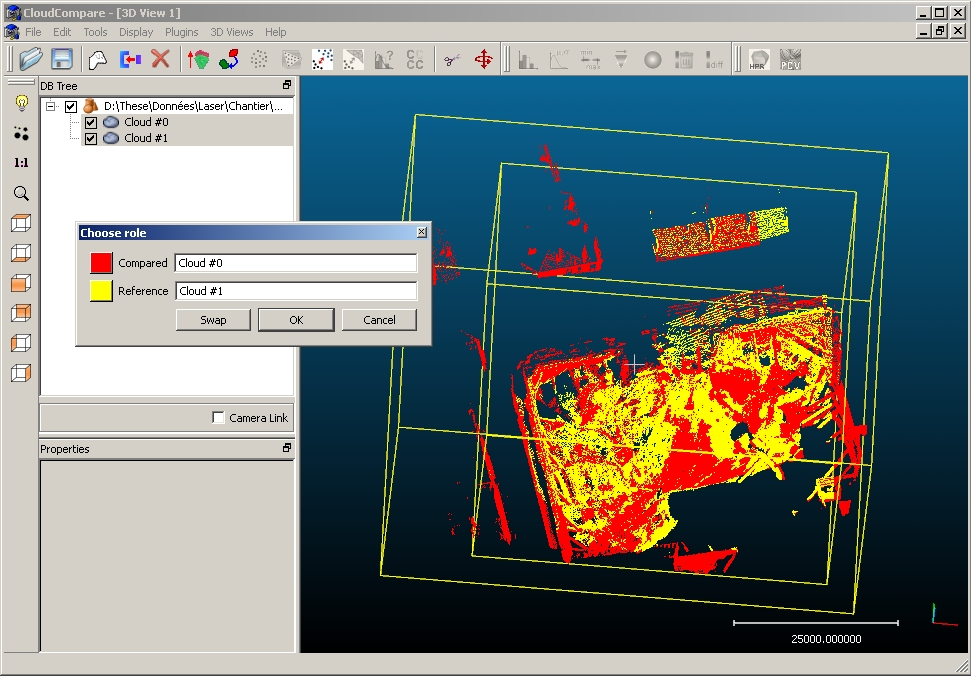
\includegraphics[width=0.9\textwidth]{Partie3_Fonctions/chooseRoleDlg.jpg}
\caption{\label{fig:chooseRoleDlg}Interface standard de choix des r�les des entit�s}
\end{center}
\end{figure}
